\documentclass[12pt]{article}
\usepackage[margin=1 in]{geometry}
\usepackage{graphicx}
\usepackage{float}
\usepackage{booktabs}
\usepackage{siunitx}
\usepackage{amsmath}


\title{Lab 6: Creating and Combining Sinusoids in MatLab}
\author{Sean Balbale}
\date{October 18th, 2024}
\setlength{\parindent}{0in}

\begin{document}

\begin{titlepage}
	\begin{center}
		\vspace*{1in}

		\Huge
		\textbf{Lab 6}

		\LARGE
		Creating and Combining Sinusoids in MatLab

		\vspace{3 in}

		\textbf{Student Name:} Sean Balbale
		\\ \textbf{Instructor:} Dr. Iman Salama
		\\ \textbf{Lab Partner Name:} Krish Gupta
		\\ \textbf{Date:} October 18, 2024

		\vfill


	\end{center}
\end{titlepage}

\newpage

\section{Introduction}
This lab focuses on the generation, analysis, and combination of discrete-time sinusoidal signals using MATLAB. 
Sinusoids, particularly sine and cosine waves, are fundamental to signal processing and electrical engineering applications, 
including biomedical signal analysis. The objective of this lab is to explore how varying parameters—amplitude, frequency, 
and phase—affect the behavior of sinusoidal signals in both visual and auditory contexts.
\newline

By generating, plotting, and combining sinusoids, we will observe the impact of these parameters on the shape, 
frequency content, and sound of the resulting signals. This hands-on approach deepens understanding of sinusoidal 
functions, which are integral to the study of circuits and signals, and prepares us for more complex applications in 
biomedical engineering and signal processing. MATLAB provides an efficient platform for simulating these signals and 
analyzing their properties, ensuring that we can accurately manipulate and study discrete-time signals.

\section{Results}
\subsection*{Part I}
\subsubsection*{A.}
\begin{figure}[H]
	\centering
	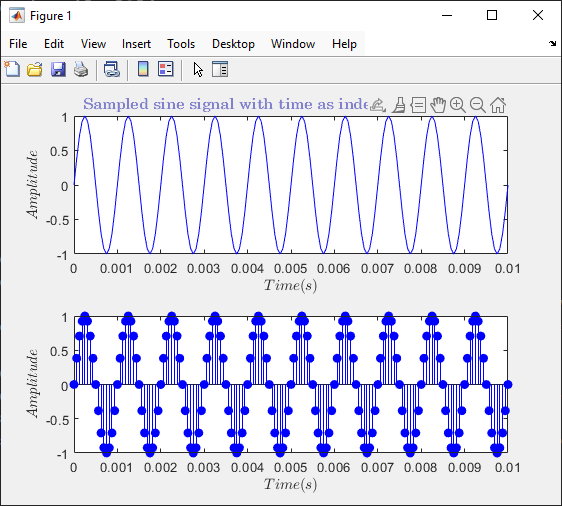
\includegraphics[width=0.5\textwidth]{fig 1a.png}
	\caption{Sinusoidal with $A$ = 1, $f$ 1 kHz, $f_s$ = 16 kHz, duration = 0.01, and Phase 0}
	\label{fig:fig1}
\end{figure}
In Figure \ref{fig:fig1}, we observe a sinusoidal signal with an amplitude ($A$) of 1, 
frequency ($f$) of 1 kHz, sampling frequency ($f_s$) of 16 kHz, duration of 0.01, 
and phase of 0. This results in 16 samples per cycle. This can be calculated through 
the formula:
\[ 
F = \frac{f}{f_s} = \frac{1000}{16000} = \frac{1}{16}
\]

\subsubsection*{B.}

\begin{figure}[H]
	\centering
	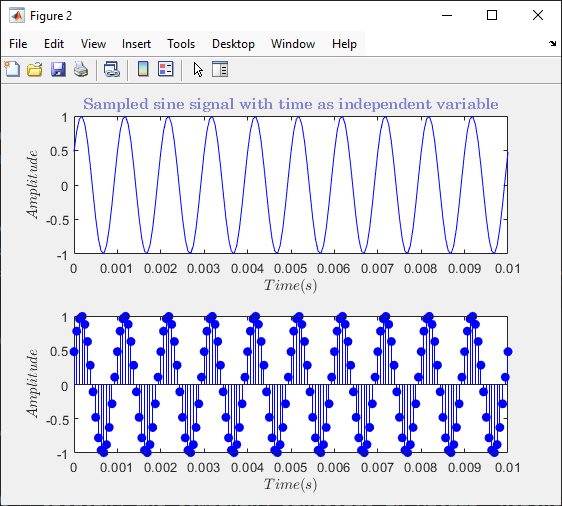
\includegraphics[width=0.5\textwidth]{fig 1b.png}
	\caption{Sinusoidal with $A$ = 1, $f$ 1 kHz, $f_s$ = 16 kHz, duration = 0.01, and Phase 0.5}
	\label{fig:fig2}
\end{figure}
As seen in Figure \ref{fig:fig2}, the sinusoidal signal has the same parameters as 
in part A, with the exception of the phase, which is now 0.5. This phase shift can be 
seen in the plot, where the signal starts at a different point in the cycle compared
to Figure \ref{fig:fig1}. The F value remains the same as in part A and there 
are still 16 samples per cycle.

\subsubsection*{C and D.}
For parts C and D, the sinusoidal signals have the same parameters as in parts A and B,
but with a duration of 1 second. The plots aren't useful for visualizing the signals,
but you can hear a beep that lasts one second. The phase shift between parts C and D
is not audible.


\subsubsection*{E.}
This part is the same as part D, but with an amplitude of 0.1. The amplitude of the
signal is reduced, resulting in a quieter beep. The phase shift is not audible.

\subsubsection*{F.}
For this part, part A is repeated but with sampling frequencies of 7000, 3000, and 
1300 Hz. 
\begin{figure}[H]
	\centering
	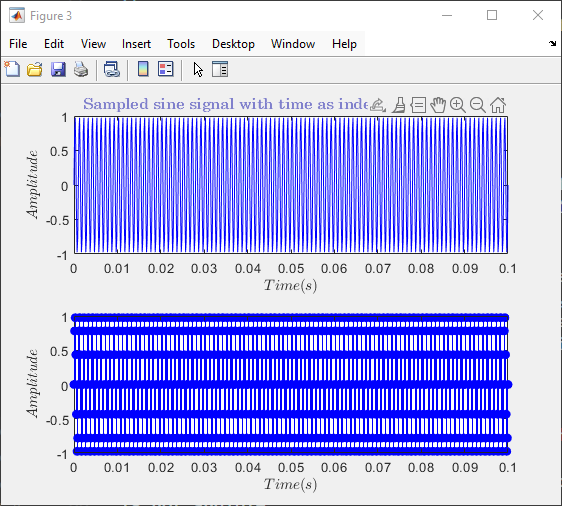
\includegraphics[width=0.3\textwidth]{fig 1f 7000.png}\hfill
	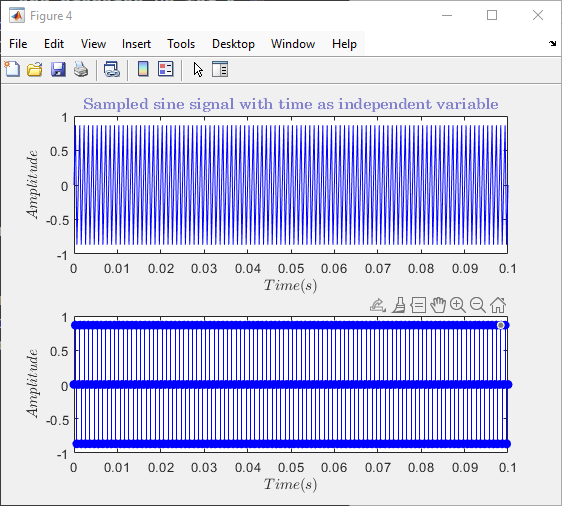
\includegraphics[width=0.3\textwidth]{fig 1f 3000.png}\hfill
	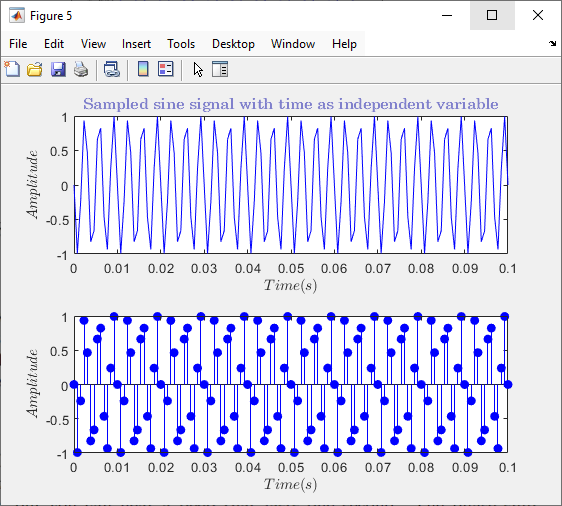
\includegraphics[width=0.3\textwidth]{fig 1f 1300.png}
	\caption{Sinusoidal with $f_s$ = 7 kHz, 3 kHz, and 1.3 kHz}
	\label{fig:fig3}
\end{figure}

As seen in Figure \ref{fig:fig3}, the sampling frequency affects the number of samples
per cycle. The signal with a sampling frequency of 7000 Hz has 7 samples per cycle, 
the signal with a sampling frequency of 3000 Hz has 3 samples per cycle, and the signal
with a sampling frequency of 1300 Hz has 1.3 samples per cycle. 

\subsubsection*{G.}
Here, part C is repeated with a sampling frequency of 7000 Hz, 3000 Hz, 1700 Hz, 
1300 Hz, and 1100 Hz. The sound of the beep decreases in quality and volume as the 
sampling frequency decreases. This is because the amount of sound data produced decreases.

\subsection*{Part II}
\subsubsection*{A.}
In this part, three sinusoidal signals are generated with frequencies of 1 kHz and 
amplitude values of 0.1, 0.3, and 1. The signals are then combined and plotted. In 
\ref{fig:fig4}, the three signals are shown. The signal with an amplitude of 0.1 is green,
the signal with an amplitude of 0.3 is blue, and the signal with an amplitude of 1 is red.
\begin{figure}[H]
	\centering
	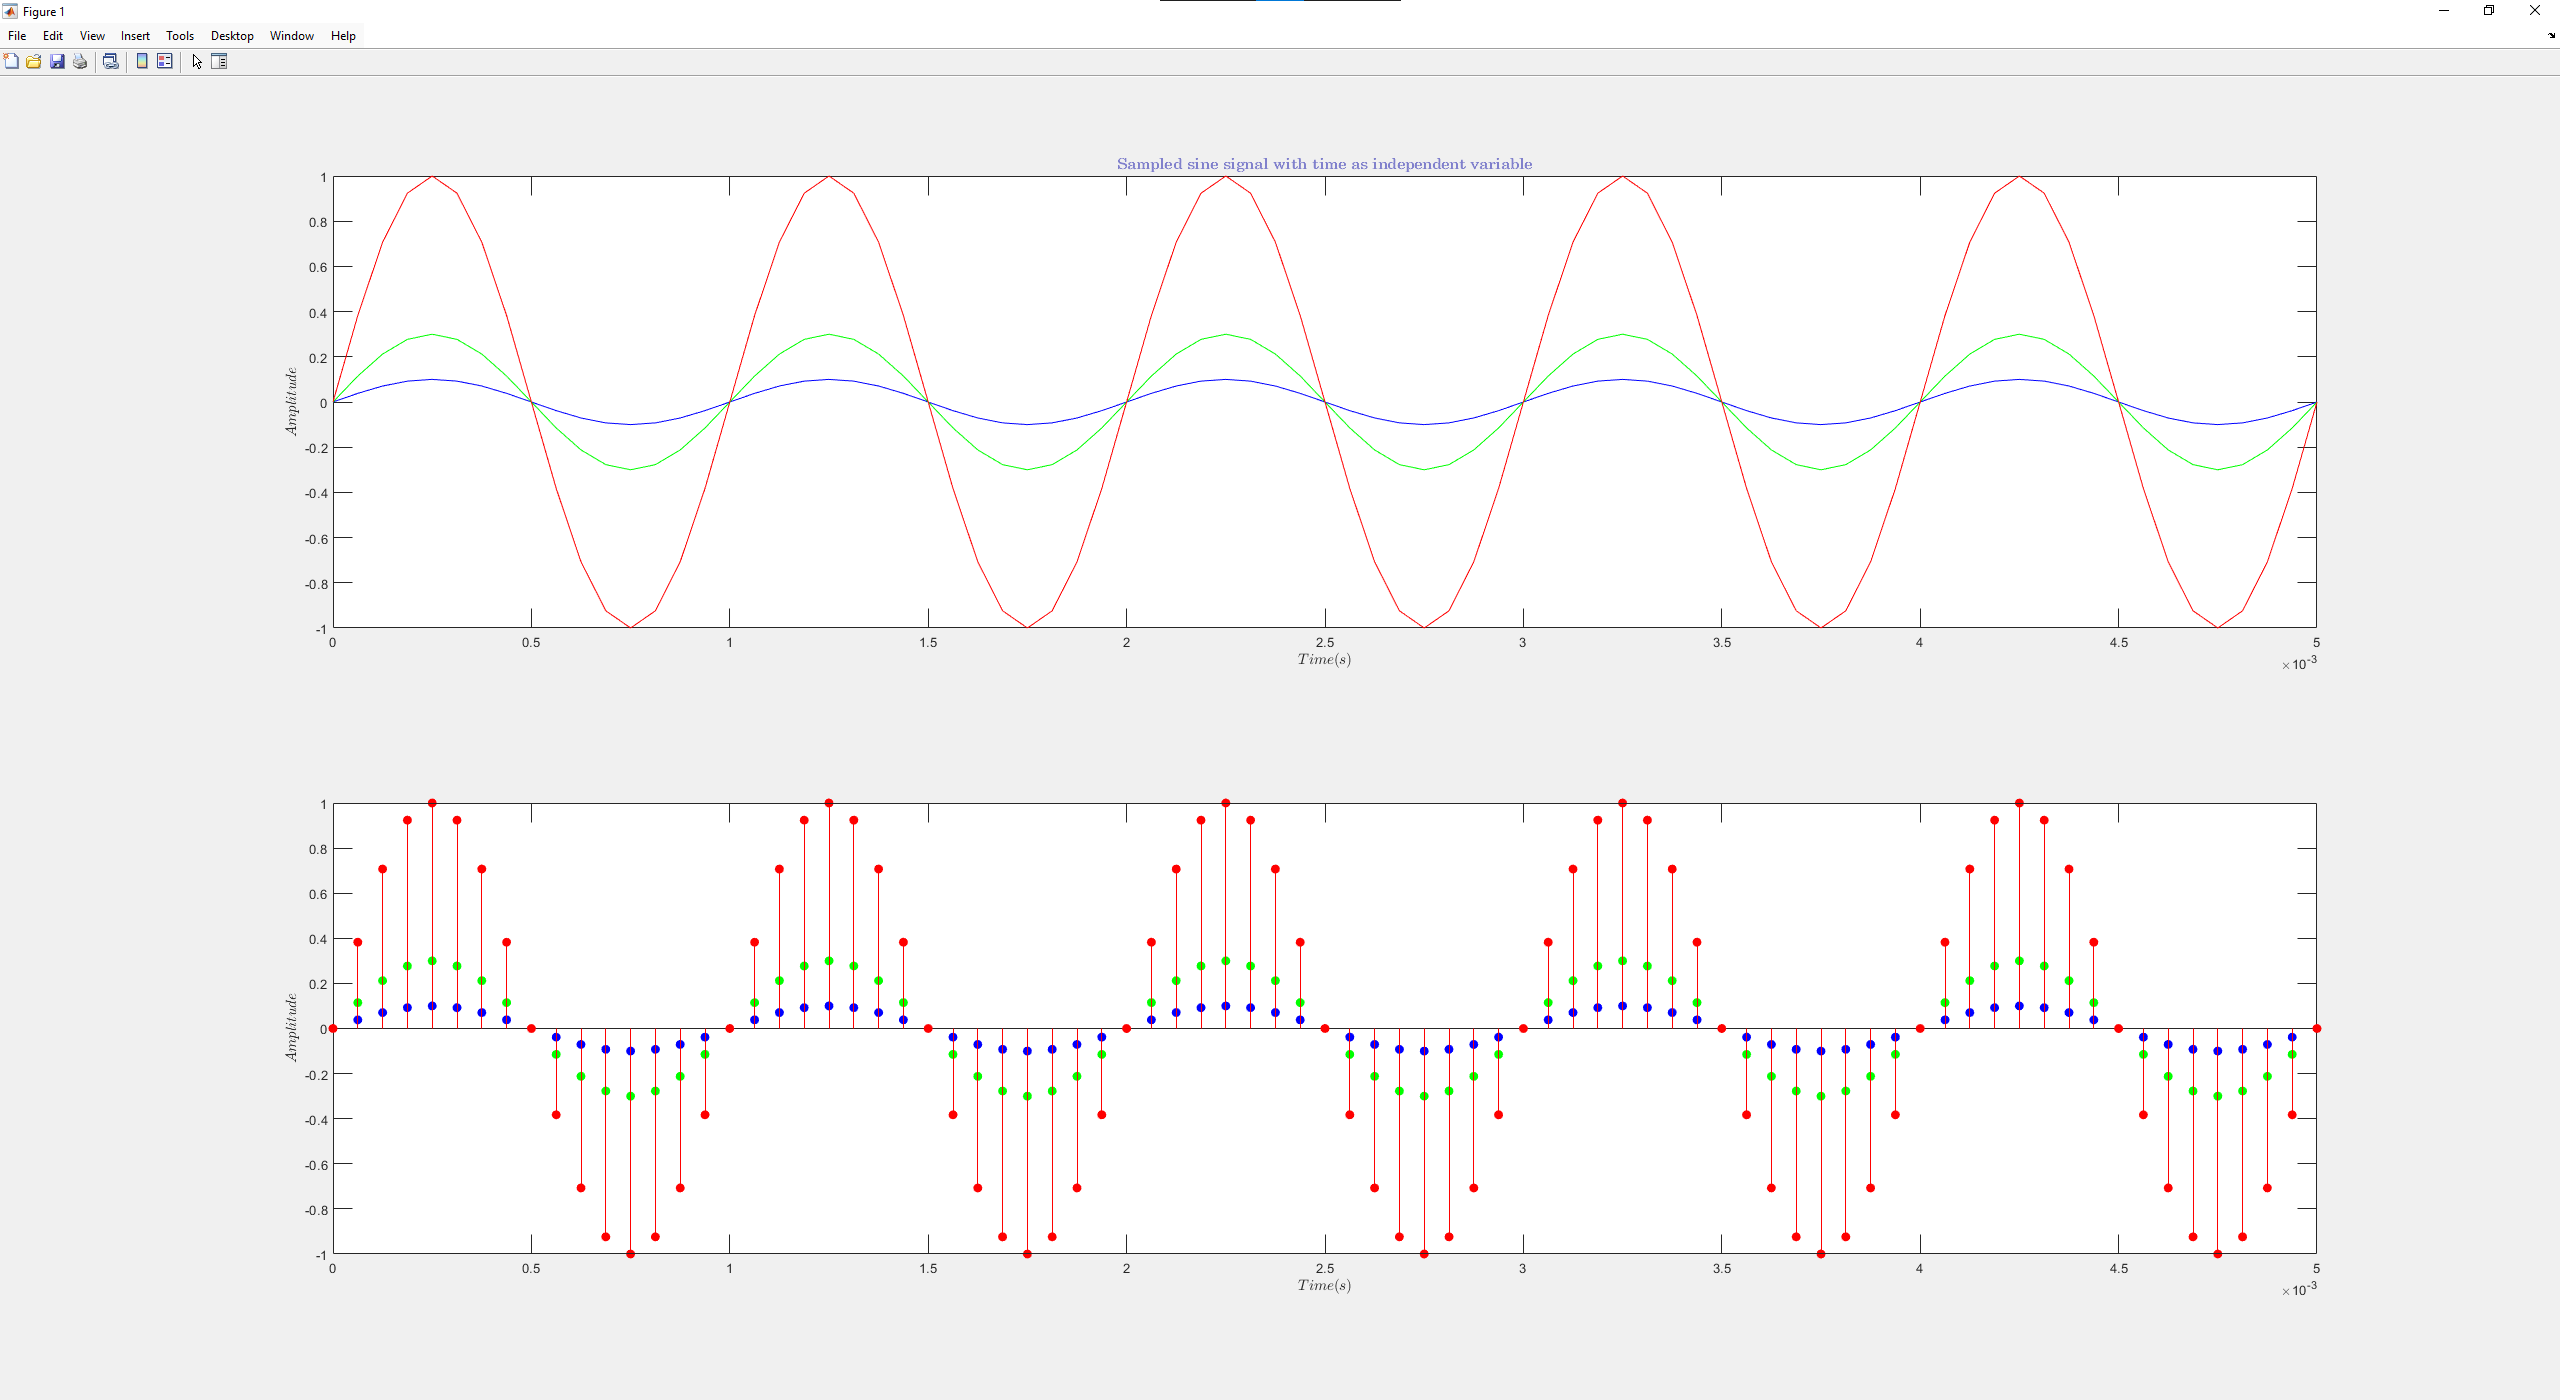
\includegraphics[width=0.5\textwidth]{fig 2a.png}
	\caption{Sinusoidal with $A$ = 0.1, 0.3, and 1}
	\label{fig:fig4}
\end{figure}

\subsubsection*{B.}
\begin{figure}[H]
	\centering
	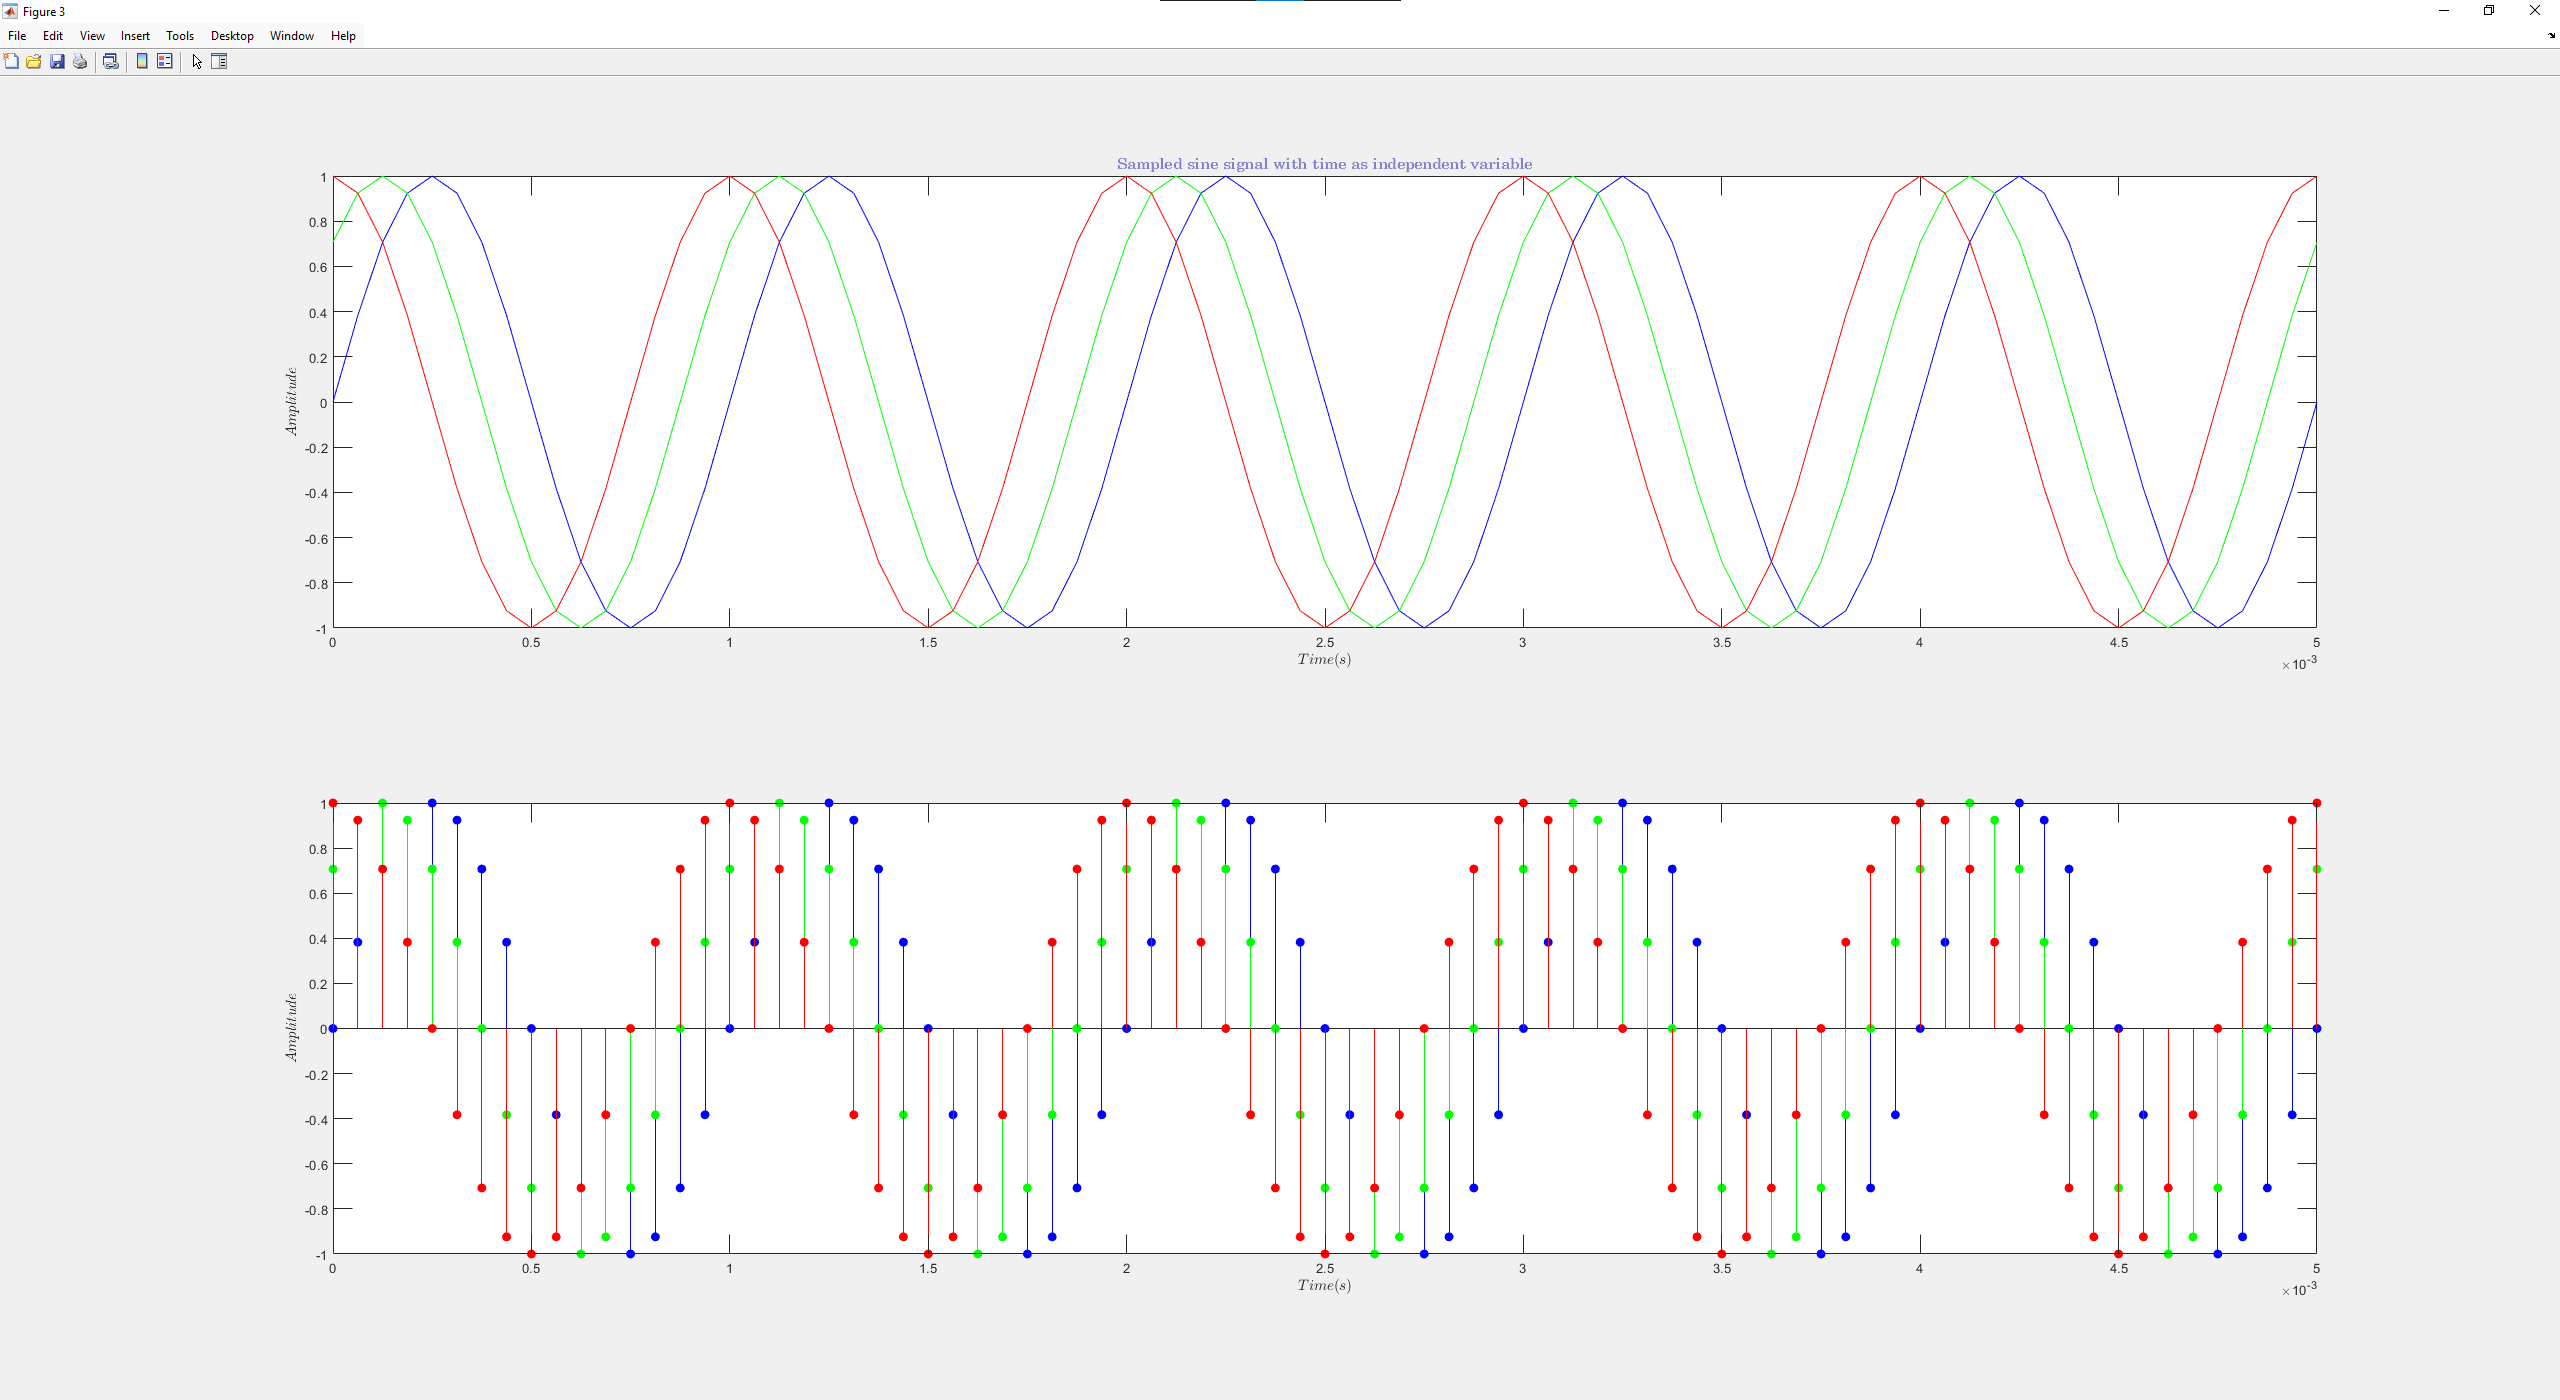
\includegraphics[width=0.5\textwidth]{fig 2b1.png}
	\caption{Sinusoidal with phase $\theta$ = 0,$\pi/4$, and $\pi/2$}
	\label{fig:fig5}
\end{figure}
In this part, three sinusoidal signals are generated with phase shifts of 0, $\pi/4$,
and $\pi/2$. The signals are then combined and plotted. In \ref{fig:fig5}. This is then
repeated with phase shifts of 0, $\pi$, and $4\pi$. The signals are then combined and 
plotted. In \ref{fig:fig6}, the signals are shown. 

\begin{figure}[H]
	\centering
	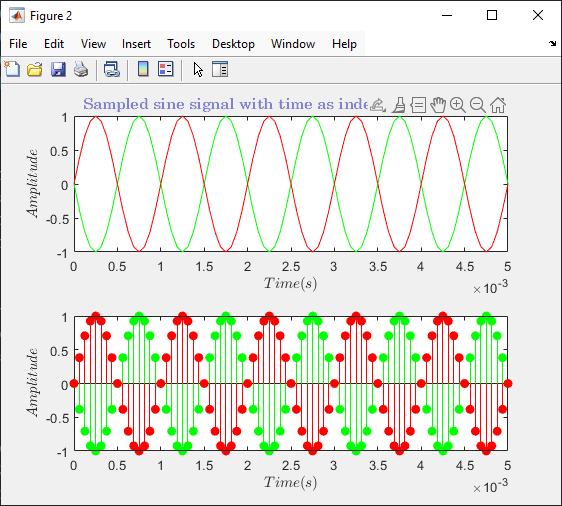
\includegraphics[width=0.5\textwidth]{fig 2b2.png}
	\caption{Sinusoidal with phase $\theta$ = 0,$\pi$, and $4\pi$}
	\label{fig:fig6}
\end{figure}

\subsubsection*{C.}
Part B is repeated but with 8000 samples. Just like the results in Part I,
the phase shift is not audible.

\subsection*{Part III}
\subsubsection*{A.}
\begin{figure}[H]
	\centering
	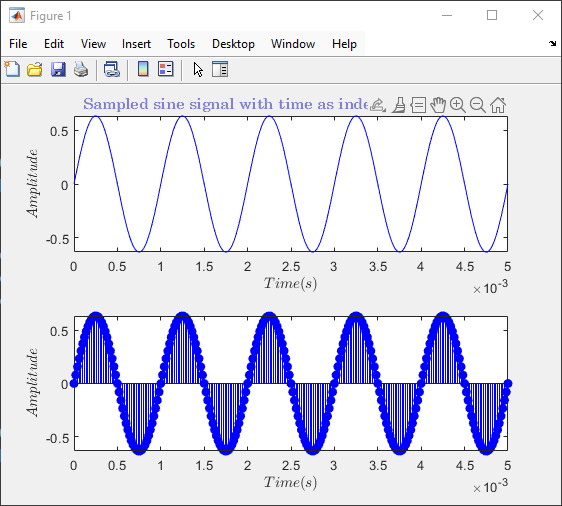
\includegraphics[width=0.5\textwidth]{fig 3a.png}
	\caption{Sinusoidal with $A$ = $\frac{2}{\pi}$, $f$ 1 kHz, $f_s$ = 5 kHz, duration = 0.005, and Phase 0}
	\label{fig:fig7}
\end{figure}
In Figure \ref{fig:fig7} we have a sinusoidal signal with an amplitude of $\pi/2$, a frequency of 1 kHz,
a sampling frequency of 5 kHz, a duration of 0.005, and a phase of 0. The signal has
a period of 5 samples per cycle. The total number of samples (N) is 250. This can be
calculated through the formula:
\[
N = f_s \times \text{duration} = 5000 \times 0.005 = 250
\]

\subsubsection*{B.}
Now a sinusoidal signal with an amplitude of $\frac{2}{3\pi}$, a frequency of 3 kHz, 
a sampling frequency of 50 kHz, a duration of 0.005, and a phase of 0 is generated and
added to the previous signal. The signals are then combined and plotted. The result is
shown in Figure \ref{fig:fig8}.
\begin{figure}[H]
	\centering
	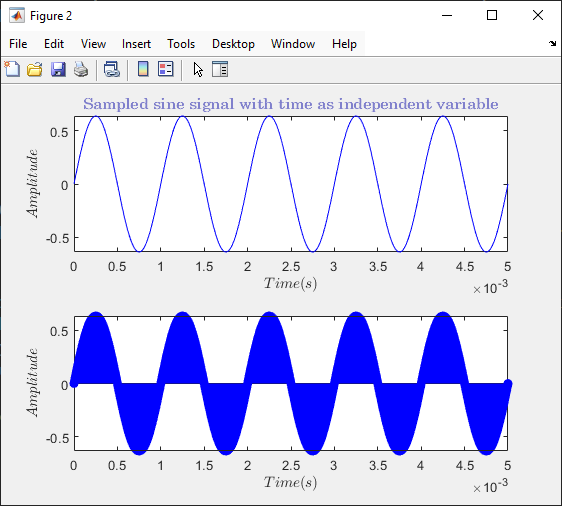
\includegraphics[width=0.5\textwidth]{fig 3b.png}
	\caption{Both Sinusoidal Signals Combined}
	\label{fig:fig8}
\end{figure}

\subsubsection*{C.}
In this part, sinusoids with amplitude $\frac{2}{n\pi}$ and amplitude $n f_0$,
where $f_0=1000 \; kHz$ and $n=5,7,9,...$ are generated. The signals are then combined
and plotted. The result is shown in Figure \ref{fig:fig9}.
\begin{figure}[H]
	\centering
	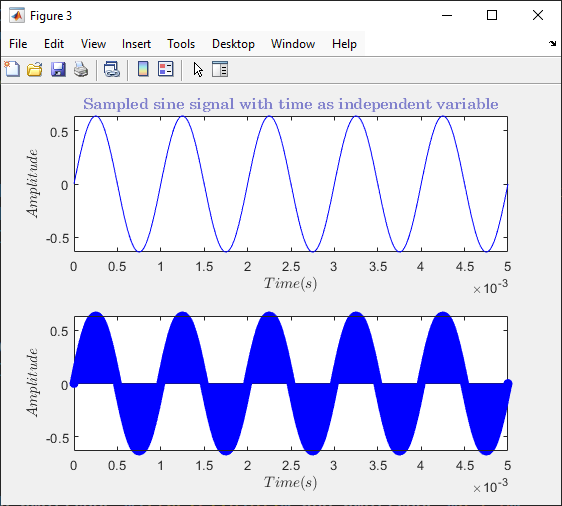
\includegraphics[width=0.5\textwidth]{fig 3c.png}
	\caption{Multiple Sinusoidal Signals Combined}
	\label{fig:fig9}
\end{figure}

\subsubsection*{D.}
Parts A and C are repeated, but with a duration of 1 second. The audio for the signals
is played. They are all beeps, but the pitch of the beep increases.

\subsection{Part IV}
\subsubsection*{A.}
You either get constructive or deconstructive interference. If the two signals are in 
phase, then you get constructive interference and the volume increases. If the two signals are out of phase, 
then you get deconstructive interference and the volume decreases.

\subsubsection*{B.}
If Part III C is repeated but the phase change ius $2\pi$, 
then the signals will be out of phase and cancel out.

\section{Discussion and Conclusion}

\subsection{Discussion}

In this lab, the generation, manipulation, and combination of discrete-time 
sinusoidal signals were explored using MATLAB, focusing on the effects of amplitude, 
frequency, and phase on the signals. Each part of the lab contributed to a deeper 
understanding of these parameters in both visual and auditory forms.
\newline

In \textbf{Part I}, amplitude, frequency, sampling rate, and phase were varied to 
observe how each affects the waveform's appearance and sound. 
The impact of the sampling frequency was particularly important. When the sampling 
frequency decreased (as seen in Part I, section F), the number of samples per cycle 
decreased, resulting in increasingly poor representations of the original signal. 
This led to noticeable degradation in both visual quality (fewer data points in each 
cycle) and auditory quality (lower fidelity). This demonstrated the importance of 
maintaining a sufficiently high sampling rate to avoid aliasing and signal distortion 
in digital systems. Moreover, the phase shifts tested (Part I, sections B and D) had 
no noticeable effect on sound but significantly altered the waveforms' visual 
representations.
\newline

\textbf{Part II} involved combining sinusoids of varying amplitudes and phase shifts. 
It was observed that amplitude affects the magnitude of the signal, while phase shifts 
influence the starting point of the wave within a cycle. By combining sinusoids with 
different amplitudes, constructive and destructive interference was effectively 
visualized. The combination of signals with different phase shifts further highlighted 
the principle of interference, where in-phase signals amplified each other and 
out-of-phase signals partially or fully canceled each other out.
\newline

\textbf{Part III} involved generating and combining sinusoids with different 
amplitudes and frequencies. A sinusoid with a frequency of 1000 Hz and an amplitude 
of \( \frac{2}{\pi} \) was combined with another sinusoid at 3000 Hz and 
\( \frac{2}{3\pi} \). The resulting waveform was more complex, containing components 
of both frequencies. 
\newline

As more sinusoids with odd harmonic frequencies (e.g., 5000 Hz, 7000 Hz) were 
added, the waveform increasingly resembled a square wave. This demonstrated the 
principle of Fourier synthesis, where complex periodic signals are constructed by 
summing sinusoids of different frequencies. When extended to 1 second, the sound 
produced became richer due to the addition of harmonic content, highlighting how 
complex sounds are synthesized in signal processing.
\newline

\textbf{Part IV} examined how constructive and destructive interference depends on 
phase relationships. Signals that were in phase resulted in constructive interference, 
amplifying the overall signal (increased volume in audio), while signals that were out 
of phase caused destructive interference, leading to diminished signals or complete 
cancellation when the phases differed by multiples of \( \pi \).
\newline

\subsection{Conclusion}

The lab demonstrated how the fundamental parameters of sinusoids—amplitude, 
frequency, phase, and sampling frequency—affect signal behavior. MATLAB 
simulations showed how these parameters influence the shape and sound of the 
signals, emphasizing the importance of phase in determining the starting point 
of a wave, amplitude in controlling signal strength, and frequency in determining 
the rate of oscillations.
\newline

Key findings include:
\begin{itemize}
    \item \textbf{Phase Shifts}: While inaudible in short-duration signals, phase shifts alter the appearance of sinusoidal waveforms.
    \item \textbf{Sampling Rate}: High sampling rates are crucial for accurately representing and reconstructing signals; lower sampling rates result in signal distortion and poor sound quality.
    \item \textbf{Combining Sinusoids}: When multiple sinusoids are combined, their relative phases and amplitudes determine whether constructive or destructive interference occurs, impacting both the visual waveform and auditory perception.
\end{itemize}

Overall, the lab reinforced essential signal processing concepts, particularly in 
the context of digital systems where discrete-time representations of continuous 
signals are critical. The use of MATLAB facilitated both the visualization and 
auditory interpretation of the signals, offering practical insights that will be 
valuable in more complex applications like biomedical signal processing.


\section{References}
 [1] Dr. Iman Salama. “Lab 6 – Creating and Combining Sinusoids in MatLab” Northeastern University. 18 October 2024.

\end{document}
